\documentclass[11pt,english]{article}
\usepackage[utf8]{inputenc}
\usepackage{geometry}
\geometry{verbose,tmargin=1in,bmargin=1in,lmargin=1in,rmargin=1in}
\setcounter{secnumdepth}{2}
\setcounter{tocdepth}{-2}
\usepackage{float}
\usepackage{amsmath}
\usepackage{graphicx}
\usepackage{setspace}
\usepackage[authoryear]{natbib}

% Fonts

%\usepackage[default,osfigures,scale=0.95]{opensans}
\usepackage[T1]{fontenc}
\usepackage{ae}

% spacing
\usepackage{multirow}

\doublespacing

\makeatletter
%%%%%%%%%%%%%%%%%%%%%%%%%%%%%% User specified LaTeX commands.
\usepackage{dcolumn}
\usepackage{parskip}
\usepackage{booktabs}
\date{}
\usepackage[ragged, bottom, multiple]{footmisc}
\usepackage[colorlinks, urlcolor=blue, citecolor=blue, linkcolor=blue]{hyperref}

\@ifundefined{showcaptionsetup}{}{%
 \PassOptionsToPackage{caption=false}{subfig}}
\usepackage{subfig}
\makeatother

\usepackage{babel}
\begin{document}
\begin{spacing}{1}

\author{
  Huhe, Narisong\\
  \texttt{naris.huhe@strathclyde.ac.uk}
  \and
  Gallop, Max\\
  \texttt{narisong.huhe@ac.uk}
  \and
  Minhas, Shahryar\\
  \texttt{minhassh@msu.edu}
}

\title{\textbf{Who Are in Charge, Who Do I Work With, and Who Are My Friends:
A Latent Space Approach to Understanding Elite Coappearances in China}\thanks{Corresponding author: Shahryar Minhas (minhassh@msu.edu).}}


\maketitle
\begin{abstract}
\begin{flushleft}

How ruling elite arrange and maintain their power-sharing is key to our understanding of authoritarian politics. We analyze the dynamics of elite power-sharing in authoritarian regimes using a network framework that embeds actors onto a low-dimensional space. We also introduce a novel dataset tracking appearances of elite Chinese Community Party (CCP) members at political events. Our framework and data allow us to disentangle three key aspects of CCP elite power-sharing: (1) who are in charge, (2) who do I work with, and (3) who are my friends. Using a latent factor network analysis of approximately 10,000 appearance records of over 200 top CCP elites from 2013 to 2017, we empirically assess these three questions by computing elites' total appearances, dyadic coappearances, and their distance in a latent social space. We test how well these three indicators fare at predicting elites' appointments to the leading small groups (LSGs) of the CCP Central Committee and the Central Government, and from that analysis are able to highlight the need to account for the indirect ties elites share.

\end{flushleft}
\end{abstract}
\end{spacing}
[Word count: 9355]
\newpage{}

%\clearpage
%\setcounter{page}{1}
\renewcommand{\footnotesize}{\normalsize}
\renewcommand{\footnotelayout}{\raggedright\doublespacing} % set spacing in footnotes
    \newlength{\myfootnotesep}
    \setlength{\myfootnotesep}{\baselineskip}
    \addtolength{\myfootnotesep}{-\footnotesep}
    \setlength{\footnotesep}{\myfootnotesep} % set spacing between footnotes
\begin{flushleft}
\setlength{\parindent}{2em}
\setlength{\parskip}{0pt}

Elite networks have been a central focus of scholars of political networks as well as social network analysis in general \citep[e.g.,][]{Knoke1993,Ward2011,Liu2015,Gross2017,Larsen2017}. Systematic exploration of these networks provides us with knowledge about complex interactions between elites (like legislators) and helps us to understand how such interactions evolve overtime \citep[e.g.,][]{Parigi2014b,Neal2018}. However, studies of elite networks in authoritarian contexts are scarce. Lacking strong and binding institutional rules, elite politics in authoritarian regimes tend to be opaque and volatile, thus limiting our ability to understand elite interactins and power sharing in these regimes. Relying on a wide range of data such as anecdotes, interviews, media coverage, and biographical archives extant studies focus mainly on identifying key elites and analyzing their social backgrounds, career patterns, and patronage ties \citep[e.g.,][]{Li1989, Levitsky2001, Albrecht2004, Perthes2004, Shih2010, Opper2015, Buehler2017}. We find few attempts to synthesize different aspects of elite dynamics, leaving us with only a fragmented perspective on elite networks in authoritarian regimes.

In this article, we propose a latent factor framework to systematically map and analyze the dynamics of elite power-sharing in authoritarian regimes. To do this we utilize elite appearance and coappearance at political events.\footnote{\citet{mahdavi_2019} also uses this approach to study relations between political elites in North Korea.} Our framework and data allow us to disentangle and synthesize three key aspects of elite power-sharing in authoritarian regimes: (1) who are in charge, (2) who do I work with, and (3) who are my friends. The question of ``who are in charge'' focuses on the power and influence of \emph{individual} elites. The answer to this question is of critical importance in authoritarian regimes where formal political institutions are vulnerable to elites' manipulation. Moving beyond individual elites, the question of ``who do I work with'' points to the \emph{dyadic} relationship between a given pair of elites (e.g., collegial ties and patronage connections), which serves as the very basis of coalitions and factions. However, a simple dyadic ``who do I work with'' approach will, we argue, overlook indirect relationships between elites and ignore information about latent coalitions. For instance, without a direct collegial or patronage connection, two elites may still belong to an unobserved coalition because of ties to a common friend. The question of ``who are my friends'' then captures such indirect \emph{latent} connections between elites. Together, by jointly considering the individual, dyadic, and latent attributes, the three ``who'' questions reveal systematic dynamics of elite power-sharing in authoritarian regimes.

Our empirical analyses and tests are focused on the Chinese Communist Party (CCP) regime. While the CCP regime has been commonly accepted as one of the most institutionalized and ``machine-like'' authoritarian regimes, many China scholars emphasize that institutional rules are epiphenomenal to elite politics \citep{Nathan1973,Tsou1976,Shih2010}. After Xi Jinping became the general secretary of CCP in 2012, the interest in elite power-sharing has been rekindled and become even more heated. Xi's first term was marked with major elite reshuffles, swift institutional changes, and wide-ranging policy alterations \citep{Miller2014b,Naughton2014,Lampton2015,Shirk2018}. These dramatic changes not only urge us to reassess CCP's intra-elite relations, but also make it an ideal laboratory to explore the three ``who'' questions. Specifically, we utilize a latent factor model \citep{Minhas2016a} to analyze a novel database that tracks approximately 10,000 appearance records of over 200 top CCP elites from 2013 to 2017. We attempt to answer the three ``who'' questions by computing elites' total appearances (i.e., ``who are in charge''), dyadic coappearances (i.e., ``who do I work with''), and, finally, their distance in a latent social space (i.e., ``who are my friends''). Our latent factor analysis of the appearance data presents a possible avenue to disentangle and synthesize key aspects of elite power-sharing in authoritarian regimes.

To probe the validity of this approach, we examine how well these three indicators fare in generating out-of-sample predictions of elites' appointments to the leading small groups (LSGs) of the CCP Central Committee and the Central Government \citep{Batke2017,Huhe2018a}. LSGs are an informal institutional arrangement of the CCP that has not been incorporated into charts of party or government organs. However, they play a pivotal role in the formulation, coordination, and implementation of decisions across different segments and levels of the CCP regime \citep{Hamrin1992,Lieberthal1992a}. LSGs not only ameliorate the regime's prolonged problem of political fragmentation, they can also be an effective vehicle for overpassing formal institutions and asserting personal influences as shown by the infamous Central Cultural Revolution Group (1966-69). Further it has been recently noted that Xi relies heavily on LSGs to push forward institutional reforms and policy changes \citep{Miller2014a,Naughton2014,Johnson2017,Lee2017,Shirk2018}. Our empirical analysis shows that while elites' total appearances are strongly associated with their appointments in LSGs memberships, their dyadic coappearances bear a much weaker association. Most importantly, the best predictor of LSG membership is our latent measure of network proximity.

Our study contributes to extant work on authoritarian politics in three important ways. First, our latent factor framework provides a possible approach to bridge and synthesize the fragmented studies of the ruling elite in authoritarian regimes. This allows us to develop a systematic assessment of their power-sharing patterns and dynamics. Second, our approach explicitly highlights and models the latent relationships between elites, which so far has received only scant scholarly attention. As revealed in our analysis of LSG appointments, the estimation of latent relations among elites may significantly improve our understanding about elite power-sharing. Finally, our study introduces a novel source of data through which to understand relations between elites in China. The appearance data enables us to systematically explore the dynamic and relational changes in elite power-sharing.

\section*{Literature Review: The Elite and Their Relationships}

How we can understand the elite and their relationships behind the facade of formal institutions has been an enduring question in social science. For instance, the ``power elite'' thesis stimulated a heated debate about the degree to which power in America is concentrated in a small cohesive group of quasi-hereditary and well-positioned elites \citep{Hunter1953,Mills2000,Dahl1961}. The debate in turn has significantly advanced our understanding about the nature of democracy \citep[e.g.,][]{Dahl1971}. In studies of authoritarian politics, scholars have been increasingly confronted by the same problem, particularly after the recent development in studies of authoritarian institutions. Although recent theoretical works, such as \citet{Svolik2012}, provide us valuable insights to link authoritarian institutions with elite contention and cooperation, we still lack a systematic framework to conceptualize and analyze the actual power-sharing dynamics in authoritarian regimes.

Our lack of a systematic framework has much to do with the highly secretive nature of authoritarian politics. It restricts researchers to employing methods such as Hunter's \citeyearpar{Hunter1953} sociometric interviews, which emerged in the ``power elite'' debate. Many studies of authoritarian elites therefore have ``been based on anecdotal and impressionistic readings of the tea leaves'' \citep[p. 137]{Ishiyama2014}. Given these limitations, a number of scholars have introduced novel empirical approaches to explore different aspects of elite politics. Such studies are particularly developed in the studies of the CCP elite, and they largely fall into two separate lines of inquiries: (1) identifying key actors (i.e., the positional approach) and (2) exploring their relations (i.e., the relational approach).

First, the positional approach focuses on \emph{individual} elites and aims to assess their de facto positions within the CCP regimes. \citet{Jaros2017} exemplifies this approach as they explore Xi's actual power and influence by examining CCP's official newspaper coverage. It is argued that the ruling elite usually rely on official media to signal their political presence and influence to the lower-level officials and the general public \citep{Huang2015b}. Their coverage in official newspapers, therefore, can be used to infer their ability to dominate the party-state. Based on their analysis of province-level party newspapers between 2011 and 2014, \citet{Jaros2017} find that Xi has received disproportionately more coverage over time, indicating a consolidating grip on power. Such large-scale quantitative analysis of texts allow us to reveal ups and downs of key elites in a dynamic way.\footnote{For similar studies, see the review of \citet{Ban2018}.} However, due to its focus on individual elites, this approach falls short in uncovering the relations between CCP elites.

The relational approach, on the other hand, examines \emph{dyadic} affinity and ties between elites. This empirical approach rests on the thesis of factional politics. It postulates that the political struggle between competing factions is the key to our understanding of CCP elite politics, with factions developing from patron-client relationships that are cultivated by a patron through the career path \citep{Pye1981,Nathan1995,Huang2000,Shih2010,Shih2012}. Empirically, scholars rely mainly on biographical archives to uncover such patron-client relationships. Based on an extensive review, \citet{Meyer2016} identify four different empirical indicators of factional ties: broad ties, complete work ties, early work ties, and restrictive work ties. They further examine how CCP elites' varying ties with the party secretary general predict their promotion into the Central Committee. Their analysis shows that while work ties with the secretary general consistently matter, non-work ties (e.g., a common educational background) sometimes could also help. In light of this, by steering our attention to factional ties associated with key patrons, this approach helps us to move beyond the power core and probe links among ruling elites.

While these two approaches provide us with important insights about elite dynamics of the CCP regime, we find that some critical problems remain unresolved. First and foremost, we still lack a conceptual framework to synthesize different insights from existing studies (e.g., dynamic changes of personal powers on the one hand and abiding factional ties between patrons and clients on the other). This in turn hinders our systematic understanding of elite power-sharing. Second and more specifically, our emphasis on key patrons and their direct clients tends to leave valuable information neglected. This is mainly due to the importance and prevalence of \emph{indirect} and \emph{non-dyadic} relationships. A client of a factional leader, for instance, could also serve as the patron for other elites.  The existence of such indirect relationships not only significantly increases the scope of factions, but, more importantly, generates a complex interdependent network of elites. Without a systemic study of such indirect relationships, we are unable to answer a series of important questions like hierarchies within factions or nuanced distinctions between apathetic and antagonistic relationships. We are limited to only looking at direct relationships rather than being able to holistically study the complete system of affinity, patronage, and antipathy. Thus we argue that  understanding elite dynamics, and thus authoritarian politics writ large, requires both new conceptual exploration and empirical strategies.

\section*{Elite Power-Sharing as a Latent Space}

In this study, we conceptualize the elite power-sharing in authoritarian regimes as a latent space. This latent space not only encompasses a collection of individual elites, it subsumes all the relationships between them, direct or indirect. In light of this, a latent space understanding allows us to synthesize both \emph{positional} and \emph{relational} attributes of the ruling elite and thus develop a systematic view about power-sharing in authoritarian regimes. Yet, despite its apparent conceptual advantages, a latent space understanding requires us to answer two critical questions: (1) how to capture it and (2) how to analyze it.

\subsection*{Political Events and Power \emph{Foci}}

How to capture the power elite and their relationship has been a key front of the power elite debate \citep{Domhoff2005}. In \emph{Who Governs? Democracy and Power in an American City} \citeyearpar{Dahl1961}, Dahl argues that the problem has risen from the obscure distinction between the legal theories of power and the realities of power: ``the American creed of democracy and equality prescribes many forms and procedures from which the actual practices of leaders diverge. Consequently, to gain legitimacy for their actions leaders frequently surround their covert behavior with democratic rituals'' (p. 89). Recognizing this, Dahl proposes to focus on political events and meetings where the actual processes of influence are at work. For instance, after observing local political nominations, Dahl finds that ``the number of persons who have participated in these decisive negotiations and influenced the outcome seems never to have been more than a half dozen in recent years'' (p. 105).

In this study, we follow Dahl's approach and turn to what we call power \emph{foci}, i.e., important political events and meetings as well as elites' appearances at them. The concept of foci is originally introduced by \citet{Feld1981} to explore people's complex and embedded social circles in a community. A focus is usually defined as a social entity or event around which joint activities are organized (e.g., voluntary organizations, hangouts, and families). Since it is around these foci that individuals organize their social relations, we can learn essential features of their latent social space by studying the observable foci. Similarly, we argue that political events like ceremonies, policy meetings, and state visits can be treated as power foci, around which the ruling elite signal and manage their power relationships. For instance, an elite's presence in a policy meeting would suggest her or his involvement in the decision-making activities and thus convey valuable information about the actual processes of influence. As the ruling elite coordinate with each other via numerous such events, we can approximate their latent space of power-sharing by examining how these foci are interconnected.

The interlocking network of power foci reveals both positional and relational attributes about the ruling elite. It is positional in its ability to uncover individual elites' relative activeness and prominence in events where the actual processes of influence are at work. Moreover, the particular patterning of an elite's appearance defines her or his points of reference in the nebulous ruling group. This is consistent with Dahl's \citeyearpar{Dahl1961} emphasis on observing decision-making activities. The interlocking foci network is also relational. Beyond specific events or individual elites, it shows how elites are connected via a variety of political events. Political elites intersect with each other within different political events, which are created based on shared policy problems or personal affinities. These links are not only able to channel important resources like information, but also can support mechanisms through which elites monitor and sanction each other.

\subsection*{Three ``Who'' Questions in a Latent Space}

How can we approximate the latent space of power-sharing from the interlocking foci network? In this study, we treat the foci network as a product of both stochastic and strategic factors. We further disaggregate the strategic factors into three questions: who are in charge, who do I work with, and who are my friends -- these correspond to the individual level characteristics, dyadic links, and latent affinities. Generally speaking, our approach can be summarized as follows: after controlling for random noise, powerful elites (i.e., who are in charge) are more likely to make appearances; elites who are in the same and related policy domains (i.e., who do I work with) are more likely to appear together; and finally elites who share latent affinities (i.e., who are my friends) are more likely to show up together. Together, the ``three'' who questions help us to approximate the latent space of elite power-sharing.

The first two who questions are quite consistent with the existing studies of elite politics. Similar to such positional studies as \citet{Jaros2017}, the question of who are in charge is focused on network dynamics that are stemmed from characteristics of individual elites. For instance, certain type of actors tend to be more active in initiating connections. In our case of elite politics, this suggests that powerful elites are more likely to preside and participate in important ceremonies and meetings. From the network analysis perspective, this greater tendency of certain actors to undertake certain behaviors is usually referred as first-order dependencies \citep{Kenny2006}. For example, we expect that Xi Jinping is simply going to make more appearances in aggregate than would a junior CCP elite. That is, if we compare two possible elites, a third person is \emph{ceteris paribus} more likely to make a coappearance with Xi than with the junior CCP elite. On the other hand, the second who question examines if two elites attend the same event. Given its focus on the observable direct and dyadic links, this question follows an approach similar to that of \citet{Shih2010}. The question of ``who do I work with'' then highlights whether there is a direct coordination and collaboration between a pair of elites.

However, what we emphasize in this study is that we cannot equate ``who do I work with'' with ``who are my friends.'' Simply using direct and dyadic links as a proxy of the latent affinity could lead to two types of errors, the incorrect rejection of a true friend and the false acceptance of a real enemy. A straightforward example of the first error is an indirect patronage relationship that involves a patron, a client, and a sub-client. If we rely solely on dyadic coappearance, we may end up wrongly rejecting the relationship between the patron and sub-client. The second error could also occur in a three-party relationship when an elite share links with two rival patrons. In this case, we could run into either a false conclusion or no conclusion at all. Provided with these possible errors, some scholars have questioned the validity of factional studies based on dyadic analyses. For example, \citet{Miller2015d}, a long-time observer of CCP elite politics, points to two problematic cases, Liu Yunshan and Li Yuanzhao, both of whom share strong ties with the competing Jiang and Hu factions. Without a consistent criterion, she argues ``in the Xi era, faction-based analyses frequently rest on assertions of factional association that are tenuous, arbitrary, and at times peculiarly fungible'' (p. 7).

In this study, we argue that the problems listed above stem from the prevalence of indirect ties in elite politics. Our approach to build on this literature involves examining the more complex and indirect relationships elites form. We thus turn to the question of ``who are my friends,'' which is commonly referred to as a third order dependency in network analysis.\footnote{Second-order dependencies refers to reciprocity, which does not apply to our case here.} Unlike first-order dependencies that are associated with attributes of individual actors, such high-dimensional dependencies usually arise from mechanisms such as homophily and stochastic equivalence. Homophily is the tendency for actors who share similar unobserved characteristics, such as similar foreign policy preferences, to be more likely to form ties with one another  than actors that do not share those characteristics. Stochastic equivalence is the idea that actors might have similar roles in the network, and thus be more or less likely to make appearances with common coalitions. If two elites in China are both prot\'{e}g\'{e}s of Xi Jinping, then they are both more likely to make co-appearances with Xi and his other prot\'{e}g\'{e}s, and less likely to make co-appearances with Xi's rivals and his rivals' prot\'{e}g\'{e}s. Therefore, a systematic study of such indirect ties helps us to understand the complex interdependencies between elites and thus provides a more accurate answer to the question of ``who are my friends.''

% To sum up, in this study we propose to estimate relations among elites through a latent space approach that allows us to better represent the dynamics of  elite power-sharing. We further argue that we can approximate this latent space by examining how power foci (i.e., political events and elites' appearance at them) are interconnected. Finally, we highlight the three who questions we need to address in this approximation. In the following parts, we introduce our empirical strategies and discuss how the approach could help shed light on the development of such informal institutions as the leading small groups.

\section*{Data}

In this study, we rely on a unique database from the China Vitae project, which traces the public appearances of CCP elites. We focus on the time period between January 1 2013 and January 1 2017, which provides us with approximately 10,000 appearance records for over 200 elites. This allows us to systematically examine the elite power-sharing in Xi's first term. It should be noted that public appearances can provide important signals to both the general public and the regime insiders.  On the one hand, CCP elites are propelled to project an image of solidarity to the general public.  This is of critical importance to the overall regime stability as the party split in late 1980s led to the regime-challenging Tiananmen movement.  On the other hand, for the regime insiders, especially lower level officials peripheral to the power center, the public appearances of top elites serve to signal important policy and political changes, which in turn are key to factional struggles and policy implementations.   In other words, public appearances of CCP needs not only to be uniform enough to show the party unity, but also to be sufficiently differentiating so as to reveal underlying elite affinities and policy priorities.

Given these competing incentives, two kinds of organizing protocols emerged, that is, “by-rank-only” and “by-invitation-only.”  Most regular and ceremonial appearances like plenary sessions of the Central Committee (CC) follow the protocol of “by-rank-only.”  The attendance in these events are determined by formal party ranks (e.g., members of the CC Standing Committee, full CC members, and alternate CC members), and the extensive media coverage on these events help to present a unitary voice of the party.  In our following analysis, we did not include events based on the protocol of “by-rank-only” for two reasons.  First, our data has been collected in Xi’s first term, and there was no reshuffle in CC.  The attendance in these events, therefore, is largely uniform, conveying little information other than party ranks.  Second, despite their extensive media coverage, the number of these regular appearances is disproportionately small compared to events of “by-invitation-only.”  For instance, the CC plenary sessions run on annual basis, and there were only four occurrences in our dataset.

Our study focuses on the events based on the protocol of “by-invitation-only,” which constitutes the large majority of public appearances of CCP elites but receives little public attention.  In sharp contrast to events of “by-rank-only,” there is no formal rules to organize these events, and the attendance is largely determined by key elites who are in charge of the specific policy domains.  For this reason, these events reflect critical political and policy changes in CCP.  To illustrate this, we can turn to two policy domains, Xinjiang and Tibet, which have 66 and 46 related entries respectively.  A closer look at these entries point to important policies differences and potential personnel changes.  Specifically, while Guo Shengkun, as the police chief, has attended multiple meetings and events related to Xinjiang, neither were invited to any meetings related to Tibet.  Similarly, Wang Yang, the Vice Premier overseeing rural affairs and poverty reduction, appeared in the Xinjiang meetings but not the Tibet ones.  On the other hand, we find Wang Yi, the Minister of Foreign Affairs, and Liu Qibao, the head of the CC Propaganda Department joined meetings related to Tibet but not Xinjiang.  Taking together, we can find these appearances help to revealing CCP’s striking policy differences in two seemingly similar domains.  While in Xinjiang CCP took an inward looking approach by focusing on public security and local economy, an outward looking approach is carried out in Tibet with the aim of winning international support.  Moreover, we find elites who were actively engaged in Xinjiang policies have gained important promotions.  In the reshuffle of the 19th CC in October 2017, Guo Shengkun was promoted to the full CC member, and Wang Yang to one of the seven members of the Politburo Standing Committee.

Table~\ref{tab:eventDesc} presents a small sample of our dataset and reports the date, the event, and elites in attendance.\footnote{Further information about the event locations, topics raised, and sources are also available.} From Table~\ref{tab:eventDesc}, we show that our dataset captures how top CCP elites structured their power relationships via a variety of political activities, ranging from the civil-military unity meeting to the China-US summit. As argued above, these power foci constitute an interlocking network of events and elites, and Figure~\ref{fig:focinet} shows how the six events in Table~\ref{tab:eventDesc} could form a simple interlocking network. Since our main focus are relationships among elites, we then extract the elite coappearance network as shown in Figure~\ref{fig:appnet}, and such coappearance networks serve as the starting point of our later analyses.

\noindent \begin{center}
\begin{table}[H]
\caption{A selected sample of political events}
\label{tab:eventDesc}
\centering
\small
\begin{tabular}{p{1in}p{3in}p{2in}}
  \\[-1.8ex]\hline
  \hline \\[-1.8ex]
   Date & Event & Attendee \\    \hline \\[-1.8ex]

  \tt{2013-01-25}  & \tt{Vice-Chairman of the Central Military Commission calls for efforts to promote unity among army, government and the people} & \tt{Zhang Gaoli, Xu Qiliang}\\
    &  &  \\
  \tt{2013-02-07}  & \tt{Xi Jinping urges \#CPC to accept criticism and be receptive to the views of non-communists} & \tt{Xi Jinping, Li Keqing, Yu Zhengsheng}\\
    &  &  \\
   \tt{2013-03-18}  & \tt{Xi Jinping endorses work of Hong Kong \#HK, \#Macao governments \#China} & \tt{Xi Jinping, Zhang Dejiang, Li Yuanchao, Yang Jiechi}\\
    &  &  \\
   \tt{2013-04-14}  & \tt{Premier stresses foresight in economic policymaking \#China} & \tt{Li Keqiang, Zhang Gaoli, Ma Kai, Liu Yandong}\\
    &  &  \\
   \tt{2013-05-20}  & \tt{Chinese Premier visits memorial of Mahatma Gandhi in New Delhi \#India \#China} & \tt{Li Keqiang, Wang Yi}\\
    &  &  \\
   \tt{2013-06-07}  & \tt{Xi, Obama meet for 1st summit \#China \#USA} & \tt{Xi Jinping, Wang Yi}\\
   ... & ...  & ... \\ \\[-1.8ex]     \hline
 \hline \\[-1.8ex]
\end{tabular}
\end{table}
\par\end{center}

\noindent \begin{center}
\begin{figure}[H]
\noindent \begin{centering}
\subfloat[Foci network\label{fig:focinet}]{\noindent \begin{centering}
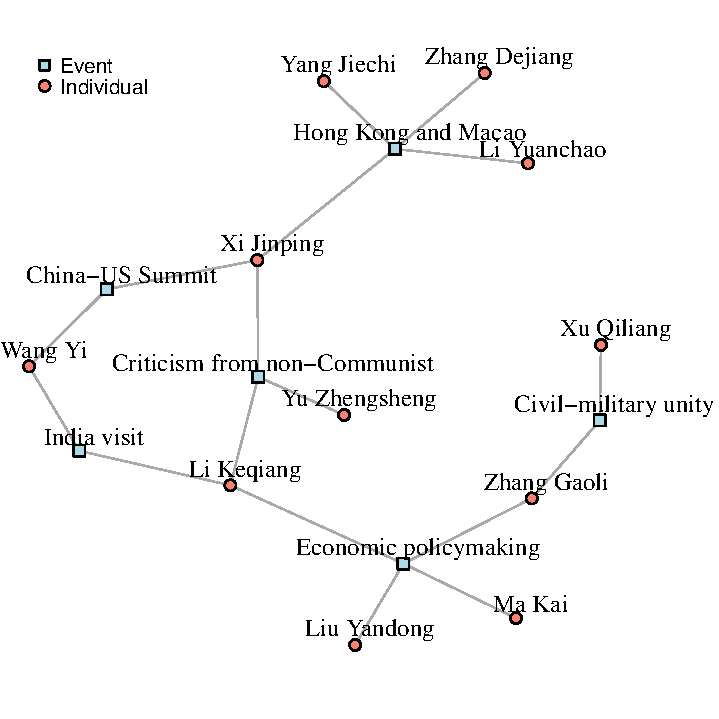
\includegraphics[width=2.5in]{data_fig1}
\par\end{centering}
}\subfloat[Appearance network\label{fig:appnet}]{\noindent \begin{centering}
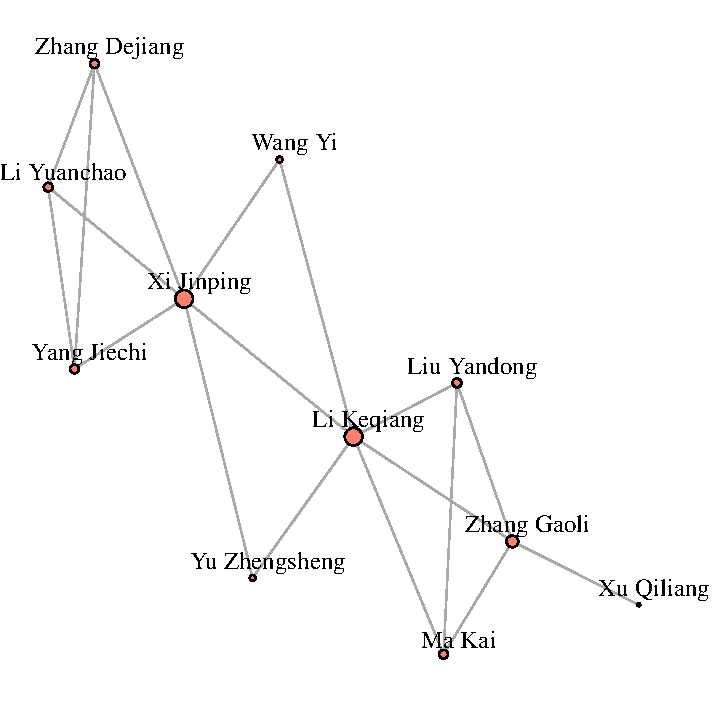
\includegraphics[width=2.5in]{data_fig2}
\par\end{centering}
}
\par\end{centering}
\caption{The interlocking networks of power foci. In the right panel, nodes are scaled by the number of total appearances.}
\end{figure}
\par\end{center}

\noindent \begin{center}
\begin{figure}[H]
\noindent \begin{centering}
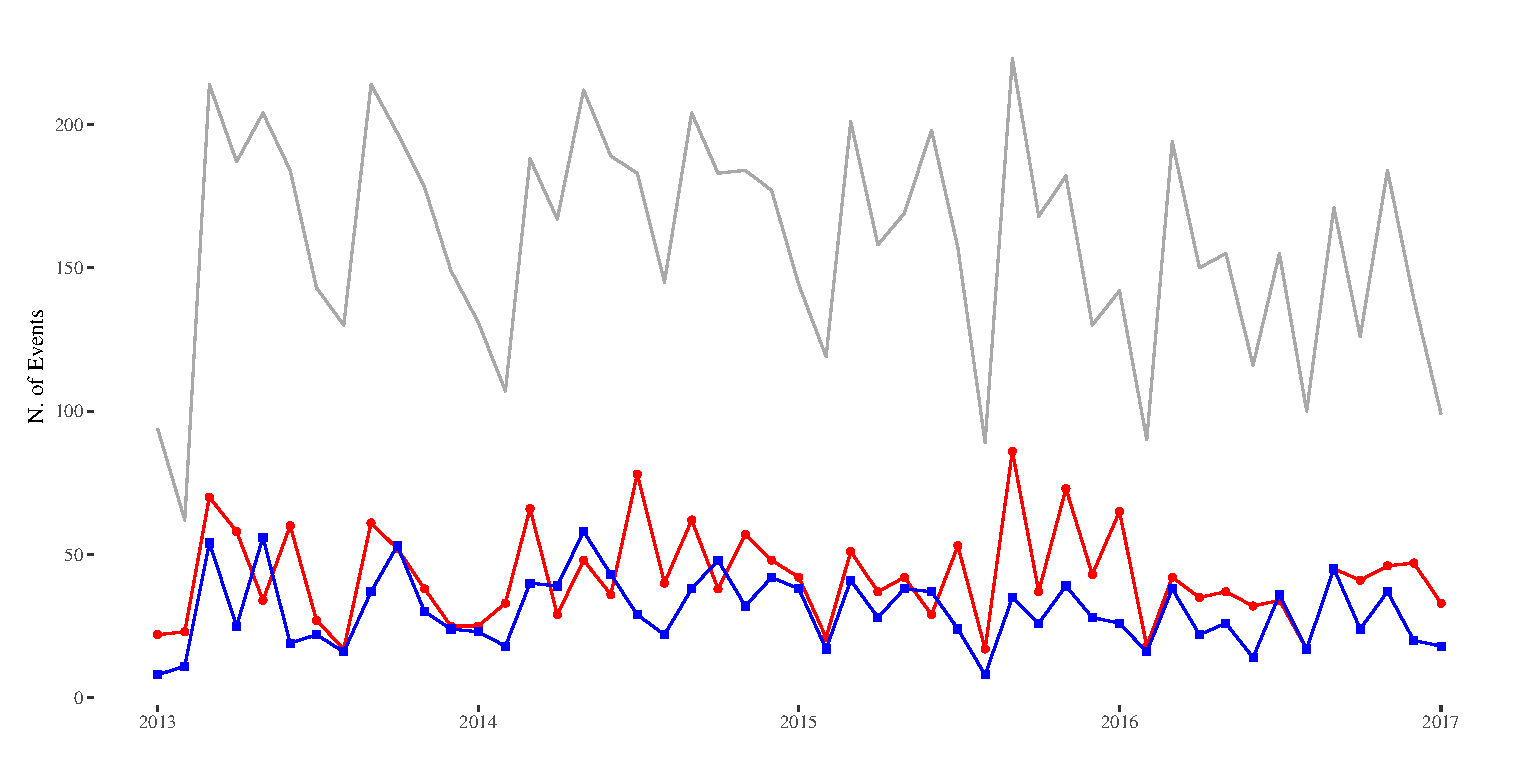
\includegraphics[width=1\textwidth]{freq}
\par\end{centering}
\caption{Total appearances (gray), Xi (red), and Li (blue). Dashed vertical lines denote the months of February and August and the dotted lines denote March and September.}
\label{fig:freq}
\end{figure}
\par\end{center}

After constructing the complete coappearance network, we can answer the questions of ``who are in charge'' and ``who do I work with'' by calculating elites' total appearances and coappearances. Figure~\ref{fig:freq} plots the total number of elite appearances (gray), as well as those associated with Xi Jinping (red) and Chinese Premiere Li Keqiang (blue) respectively. A quick examination shows a consistent annual pattern. There are notably fewer elite appearances in February and August (denoted by vertical dashed lines), and their activities peak in March and September (denoted by dotted lines). While the low points in the Spring are mainly due to the Chinese new year, the high points in August accord with elites the CCP's tradition of summer meetings at Beidaihe \citep{Miller2014c}. A comparison of Xi and Li's appearances points to some interesting changes. In 2013 and 2014, we can find that their total appearances frequently intersected. Yet starting from 2015 Xi has made markedly more appearances. This corroborates with \citet{Jaros2017} that Xi has significantly consolidated his power in his first term.

In Figure~\ref{fig:coappFreqs}, we contrast two pairs of coappearances, Xi-Li and Xi-Zhang.\footnote{Zhang Gaoli was one of the seven members of the Politburo Standing Committee, who also served as the first-ranked Vice Premier.} In Figure~\ref{fig:Xi_Li},  the red line denotes the number of times Xi-Li coappeared at an event as a share of  Xi's total appearances. The dashed blue line also denotes the number of Xi-Li coapperances, but as a share of Li's total appearances. From Figure~\ref{fig:Xi_Li}, we find that the two lines overlapped a lot throughout the four years, and their shares of coappearances have declined over time. In other words, for both Xi and Li, their coappearances account for similar weights in their total activities, though they are gradually departing away from each other. However, Xi-Zhang coappearances in Figure~\ref{fig:Xi_ZG} show a different trend. Xi-Zhang coappearances are highly asymmetrical. The share of their coappearance is markedly more salient for Zhang, indicating the extent to which Zhang is overshadowed by Xi.

\noindent \begin{center}
\begin{figure}[H]
\noindent \begin{centering}
\subfloat[Xi and Li\label{fig:Xi_Li}]{\noindent \begin{centering}
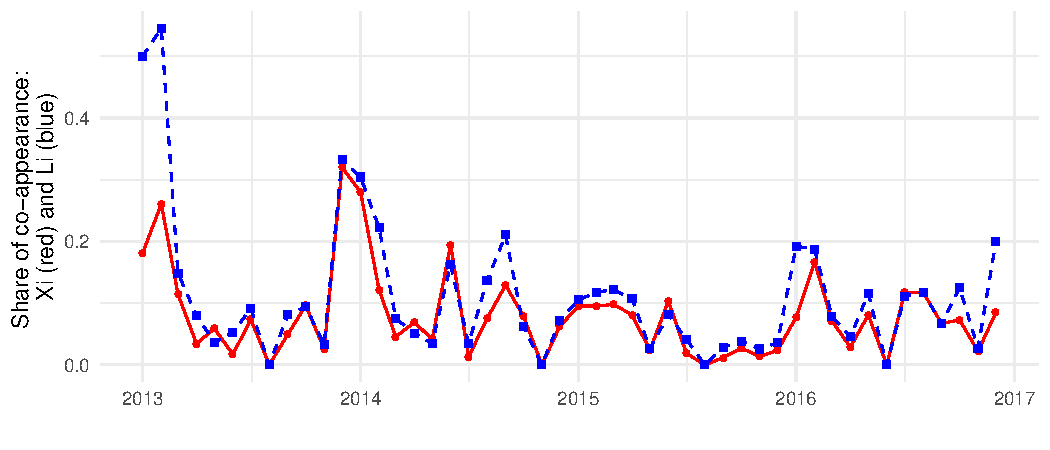
\includegraphics[width=.8\textwidth]{Xi_Li}
\par\end{centering}
}
\par\end{centering}
\noindent \begin{centering}
\subfloat[Xi and Zhang\label{fig:Xi_ZG}]{\noindent \begin{centering}
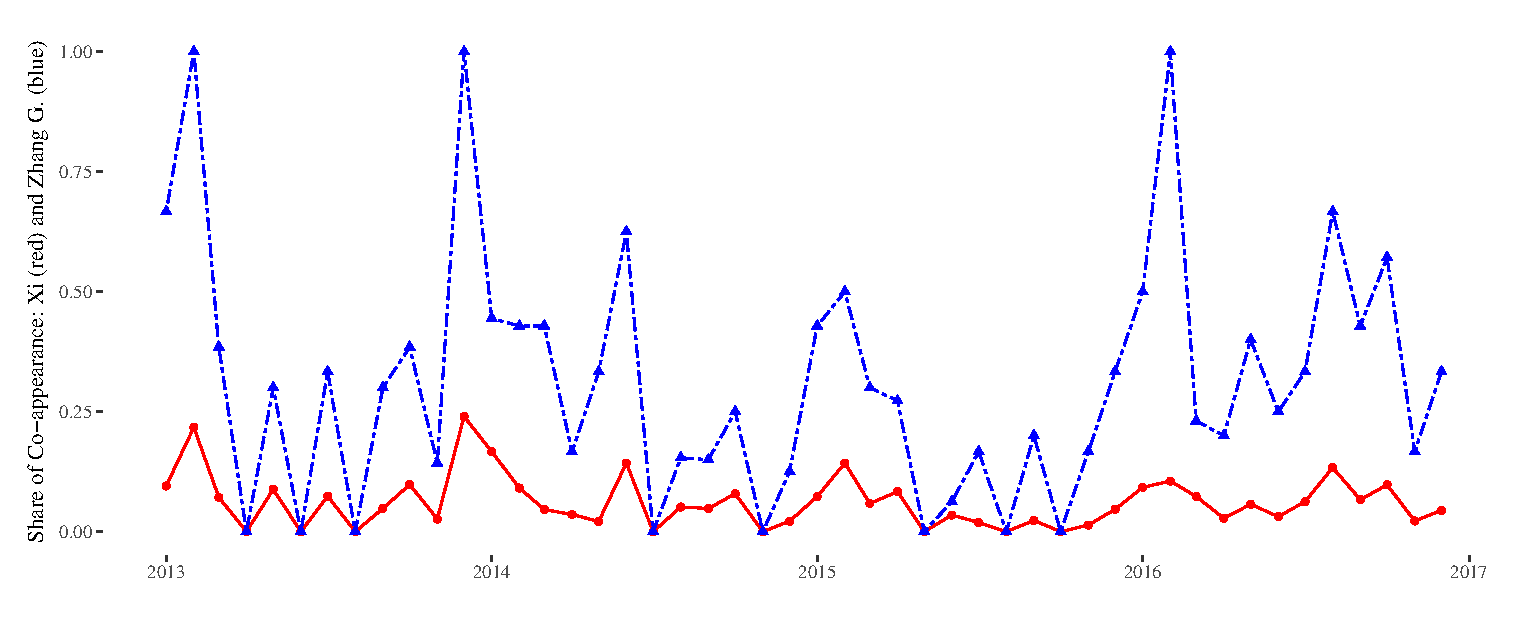
\includegraphics[width=.8\textwidth]{Xi_ZG}
\par\end{centering}
}
\par\end{centering}
\caption{Share of coappearances among total appearances for Xi (red) and Li and Zhang (blue).}
\label{fig:coappFreqs}
\end{figure}
\par\end{center}

Finally, we plot the complete coappearance network in Figure~\ref{fig:fullCoappNet}. It shows that the set of interactions captured in the coappearance network form  a complex system. While there are a few actors towards the right that only appear with one or two other actors, most fall into the broader interconnected system at the left of Figure~\ref{fig:fullCoappNet}. Moreover, within the broader interconnected component, we can find a number of patterns. First, not surprisingly, Xi Jinping and Li Keqiang are positioned towards the center of the network because of their institutional importance. However, around that central system we can see a number of sub-groups. For example, Wu Shengli, Zhao Keshi, Wei Fenghe, Ma Xiaotian, Zhang Yang, and Fang Fenghui were each high ranking military officers and their proximate positioning in the visualization indicates that they coappear with one another frequently.%\footnote{Actors are positioned in this visualization using the Fruchterman-Reingold algorithm \citep{fruchterman:reingold:1991}. These types of algorithms use information contained within the structure of the network itself to construct depictions of graphs. A straightforward way to understand how they work is to think of nodes connected by edges as particles that are attracted to each other, and nodes that are unconnected as particles that repulse each other. These types of algorithms simulate a system in which nodes pull and push upon each other until they reach an equilibrium position.}

\begin{figure}[ht]
\centering
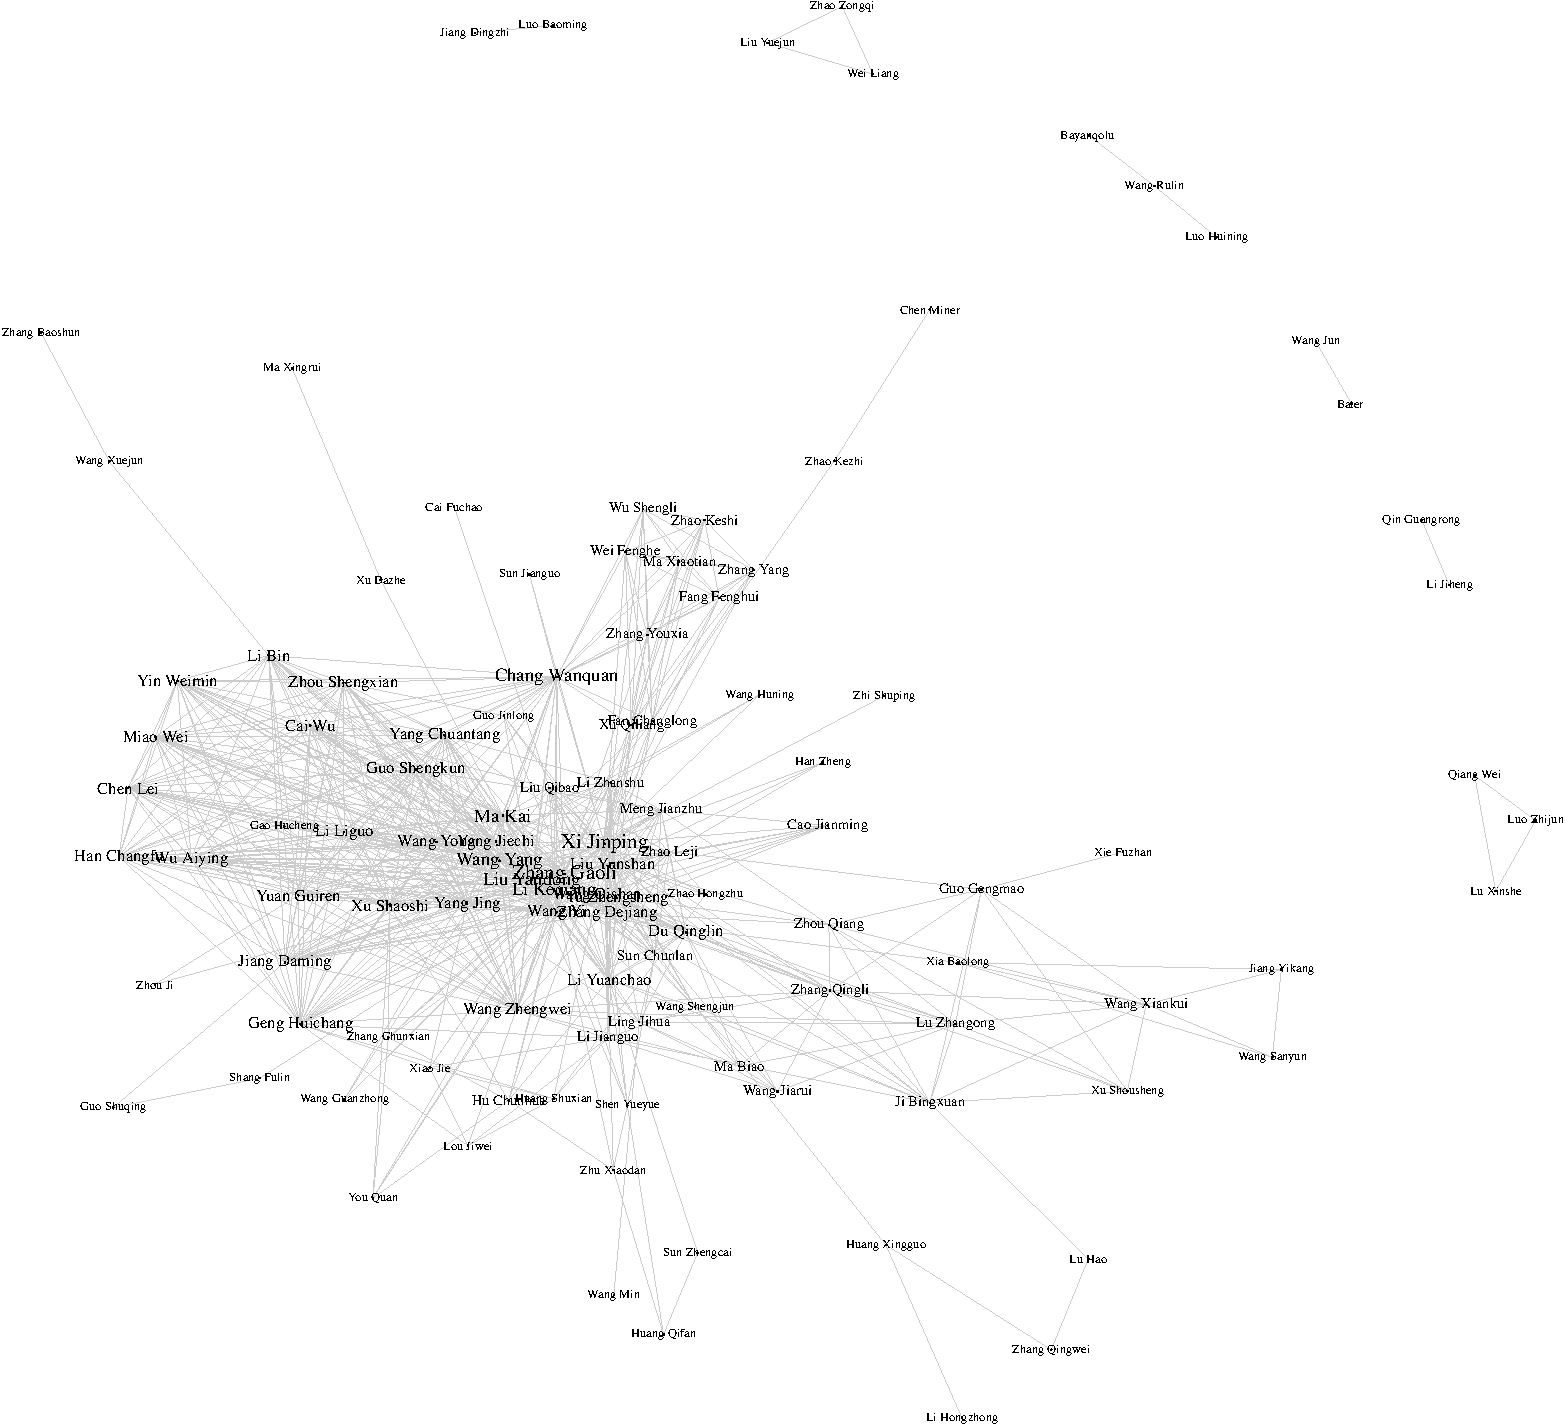
\includegraphics[width=.9\textwidth]{dvViz_names2}
\caption{The complete coappearance network. Names of elites depicted in the network are scaled by their number of appearances and edges between actors indicate that they appeared together at an event.}
\label{fig:fullCoappNet}
\end{figure}

Many such sub-groups like this appear in this visualization and this points to the fact that there is notable higher order structure within this system that may be missed by just examining direct dyadic ties. One way to quantify such higher order structures is a transitivity statistic.\footnote{A relation between a set of actors is transitive (i.e., a triangular relationship), if every time that $i$ and $j$ have a tie and $j$ and $k$ have a tie, then $i$ and $k$ will have a tie.} Here we utilize the clustering coefficient, which is a measure of the degree to which nodes in a network cluster together.\footnote{The clustering coefficient is calculated as follows, where $G$ represents the network being studied, $C=\frac{tr(G^{3})}{\sum_{i\neq j}(G^{2})_{i,j}}$.} A significant amount of higher order structures  leads to a high clustering coefficient. In our case of the CCP elite coappearance network, we find that the statistic is 0.67 on a scale from 0 to 1, indicating that a large proportion of potentially closable triads are actually closed. In the following section, we discuss our approach to systematically estimate latent affinities between actors in a network with higher order dependencies.

\section*{Latent Factor Analysis}

To answer the question of ``who are my friends,'' we utilize a latent factor model (LFM) \citep{Hoff2005,Minhas2016a}. The LFM positions actors in a $k$ dimensional latent vector space based on third order dependence patterns. In this space, actors whose vectors point in similar dimensions are more likely to share similar preferences and be members of the same latent coalitions. The angles between these vectors then provides a measure of the extent to which the preferences and factional links are similar. Given its ability to capture latent affinities between interconnected actors, LFM has been used to infer state foreign policy preferences \citep{gallop:minhas:2018}.

More formally, we conduct the analysis as follows. We treat our coappearance network as an $n\times n$ matrix, where $n$ denotes the number of elites, and the matrix cell $y_{ij}$ represents the number of coappearances between elite $i$ and elite $j$.\footnote{It should be noted that the coappearance data is symmetric and so $y_{ij}=y_{ji}$ for all $i,j$. The approach we describe below has already been generalized to the case where $y_{ij}\neq y_{ji}$.} To obtain the latent affinities between elites (i.e., a lower-dimension relational measure), we then have an LFM as follows,
\begin{align}
Y & =f(\theta)\\
\theta & =\beta^{\top}\mathbf{X}+Z\\
Z & =M+E\\
M & =U\Lambda U^{\top}
\end{align}
where $u_{i}\in{\rm I\!R^{k}}$ and $\Lambda$ is $k\times k$ diagonal matrix. $f(.)$ is a general link function corresponding to the distribution of $Y$ (in our case the coappearance count), and $\beta^{\top}\mathbf{X}$ is the standard regression term for dyadic and nodal fixed effects.\footnote{For the purpose of parsimony we abstain from using fixed effects in this study.}

The LFM accounts for network interdependencies is by decomposing the error term $Z$. \citet{Hoff2008} notes that we can write $Z=M+E$, where the matrix $E$ represents noise, and $M$ is systematic effects representing first and third order dependencies. We factorize the multiplicative effects into the product of two simpler matrices, $U\Lambda U^{\top}$. Under this framework a vector of latent characteristics are thus estimated for each actor, $u_{i}=\{u_{i,1},\ldots,u_{i,k}\}$. Similarity in the latent factors between two actors, $u_{i}\approx u_{j}$, corresponds to how stochastically equivalent they are and the diagonal entries in $\Lambda$, $\lambda_{k}>0$ or $\lambda_{k}<0$, determine the level of homophily (or heterophily) in the network \citep{Minhas2016a}.

For our interest in latent affinity, the key output is $U\Lambda U^{\top}$, where $U$ is an $n\times k$ matrix that represents each actors vector in the $k$-dimensional latent network.\footnote{We estimate a 2-dimensional latent factor space for our application.} It captures the effect of stochastic equivalence and homophily on official appearances. But a caveat in interpreting this space is that it is non-Euclidean, as the actor vectors are embedded within a $k$-dimensional hyper sphere. We thus cannot simply use distances in this space as a measure of latent affinities. Rather, the important measure here is an actor's vector in this space, and the similarity between the vector of one actor and another.

\noindent \begin{center}
\begin{figure}[H]
\noindent \begin{centering}
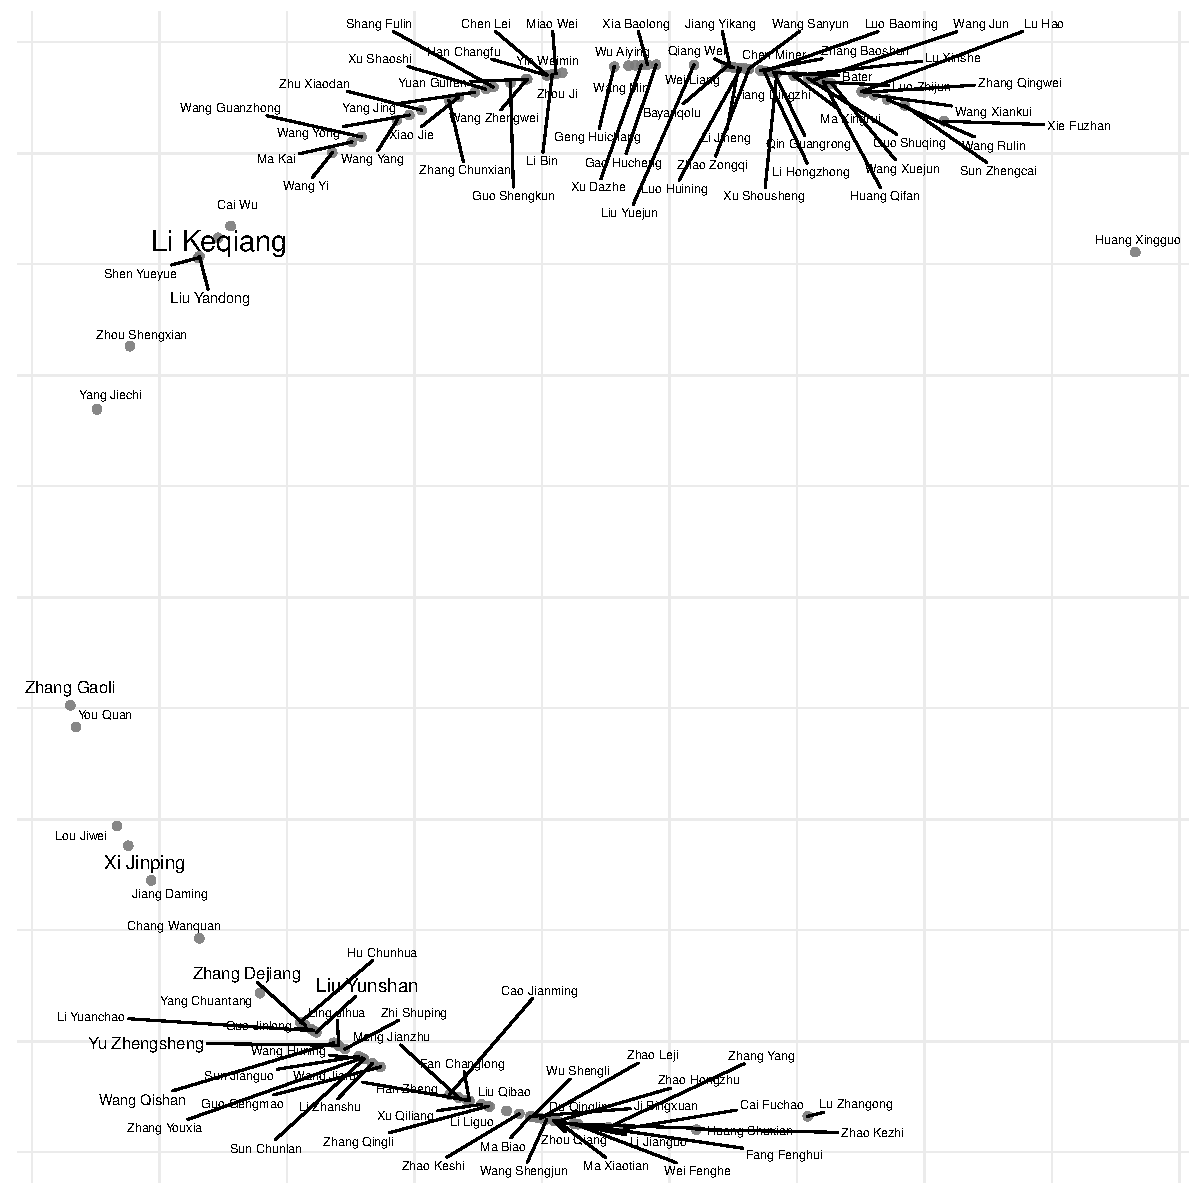
\includegraphics[width=5in]{uViz}
\par\end{centering}
\caption{Visualization of the AME latent factor space. Actors that cluster together in this space are more likely
to interact with one another.}
\label{fig:uv}
\end{figure}
\par\end{center}

Comparing the similarity between two elites, $\{i,j\}$, can be accomplished by comparing the direction to which their respective factor vectors point. A commonly used metric for this sort of problem is the cosine of the angle formed by the latent vectors of both actors.\footnote{The method is well developed in the recommender system literature of computer science. It is calculated in the following way, where $u$ represents the $n\times k$ matrix of actor vectors, $\text{Latent angle distance}_{ij}=\frac{u_{i}\cdot u_{j}}{||u_{i}||\cdot||u_{j}||}*(-1)$. } We refer to this distance metric as latent angle distance. More concretely, if the estimated latent vectors of two actors are in the same direction, they are apt to have made appearances with similar partners. We measure this by looking at the absolute distance of the angles created by each officials position and the center of the latent network, and the results are plotted in Figure~\ref{fig:uv}. Our latent angle distance measure is bounded between -1 and 1, where higher values point towards greater dissimilarity in appearance patterns.

\noindent \begin{center}
\begin{figure}[H]
\noindent \begin{centering}
\subfloat[18th Poliburo (2012-17)\label{fig:uv18}]{\noindent \begin{centering}
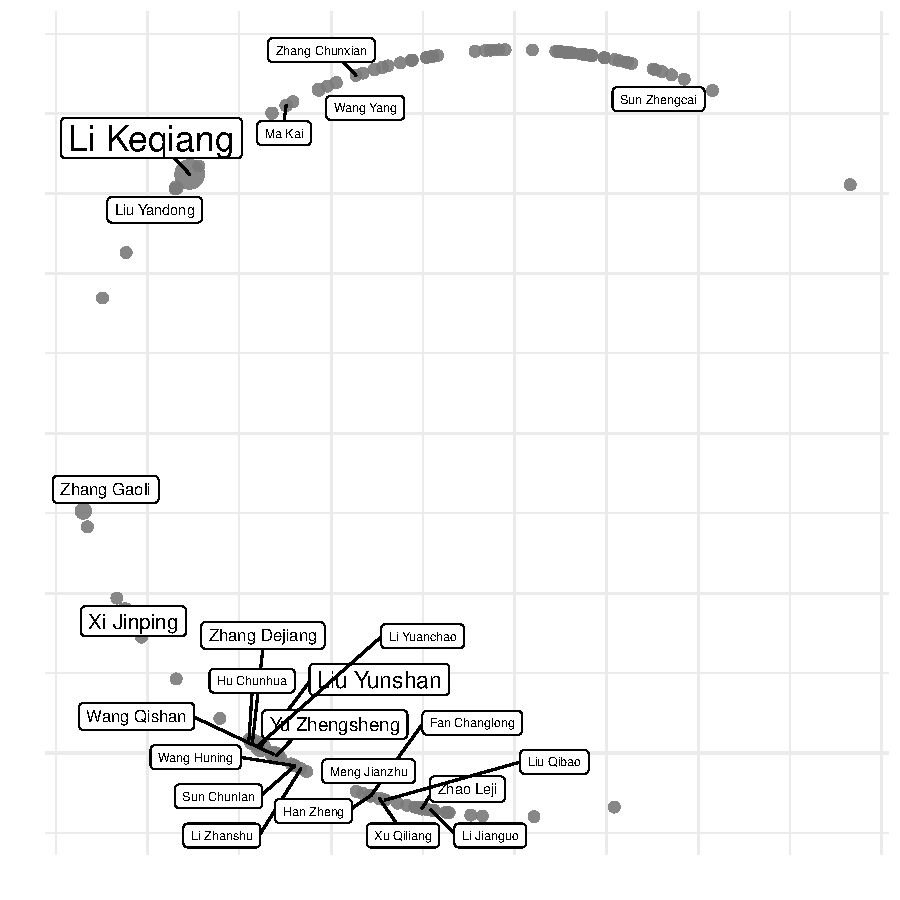
\includegraphics[width=3.25in]{politSC18}
\par\end{centering}
}\subfloat[19th Poliburo (2017-)\label{fig:uv19}]{\noindent \begin{centering}
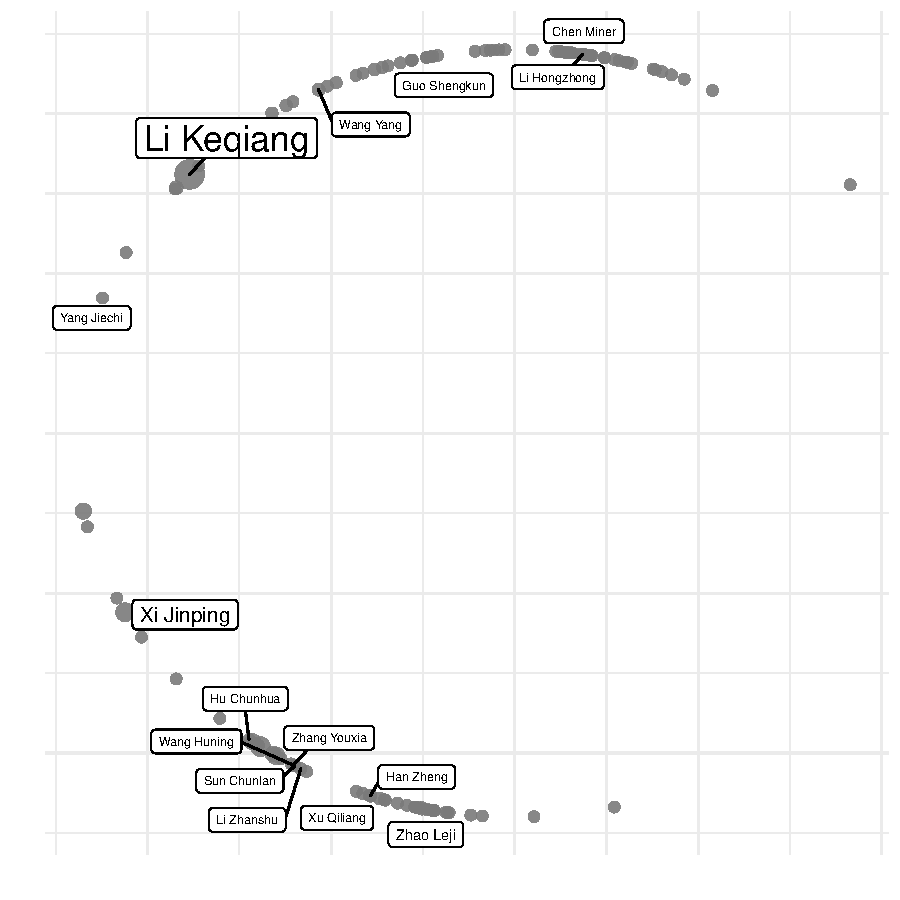
\includegraphics[width=3.25in]{politSC19}
\par\end{centering}
}
\par\end{centering}
\caption{Slices of the latent factor network with key actors highlighted from the 18th and 19th Politburo.}
\label{fig:uvSlices}
\end{figure}
\par\end{center}

In Figure~\ref{fig:uv}, we find CCP elites in our dataset fall into two clusters that are centered around Xi (i.e., the lower cluster) and Li (i.e., the upper cluster). To gain a better view about key elites, we present the slices of Politburo members of the 18th and 19th Central Committee in Figure~\ref{fig:uvSlices}. First, the 18th Politburo members as shown in Figure~\ref{fig:uv18} are also divided into the two clusters. More interesting, while the other three Vice Premiers (i.e., Liu Yandong, Wang Yang, and Ma Kai) are sided with Li, the first Vice Premier Zhang Gaoli is much closer to Xi. Second, the majority of Politburo members in Figure~\ref{fig:uv18} are clustering around Xi. Particularly, the two military members, Xu Qiliang and Fan Changlong, are also in the lower cluster. This dominant Xi cluster is consistent with findings of \citet{Jaros2017}. Third, Figure~\ref{fig:uv18} also points an outlier elite in the upper left corner, Sun Zhengcai, who is a remote member of the Li cluster. However, Sun is almost diagonal to Xi, that is, a position farthest possible from Xi in the latent space. Our data points stop on January 1st 2017, and seven months later Sun was abruptly removed from his office as the party secretary of Chongqing. Finally, Figure~\ref{fig:uv19} plots members of 19th Politburo who were elected over ten months after our last data point. It shows that how this approach is able to pick up potential changes in the Politburo. Together, the above findings suggest our approach suffice to meet satisfactory face validity.

\section*{Leading Small Groups}

To provide a more robust test of the validity of our approach, we examine elite appointments in the Leading Small Groups (LSGs). Following \citet{Huhe2018a}, we focus on LSGs at the national level, that is, the Central Committee (CC) LSGs and the State Council/Central Government (SC) LSGs. LSGs play a pivotal role in gluing the fragmented CCP regime together \citep{Hamrin1992}. As an informal arrangement, LSGs are less restrained by formal regulations and can be strongly influenced by the elites who preside them. An LSG creates an enormous confluence of leadership over various state apparatuses within one small body. Recognizing this, \citet{Lieberthal1992a} argues that ``at {[}the national{]} level, the {[}LSG{]} system is highly personal. \ldots There is \ldots a great deal of informal contact and maneuvering, with control over the various `leading groups' an important prize in the political jockeying in the capital'' (p. 14). Huhe and Stepan's \citeyearpar{Huhe2018a} study of LSGs in Xi's first term also reveal that the appointments in CC and SC LSGs are highly skewed. While a majority of LSGs appointees are affiliated with only one LSG, a few elites concurrently sit in different LSGs. And this trend is particularly evident in CC LSGs. Figure~\ref{fig:lsgNet} then shows how 242 CCP elites are linked via 19 CC LSGs and 16 SC LSGs \citep{Batke2017,Huhe2018a}.

\noindent \begin{center}
\begin{figure}[H]
\noindent \begin{centering}
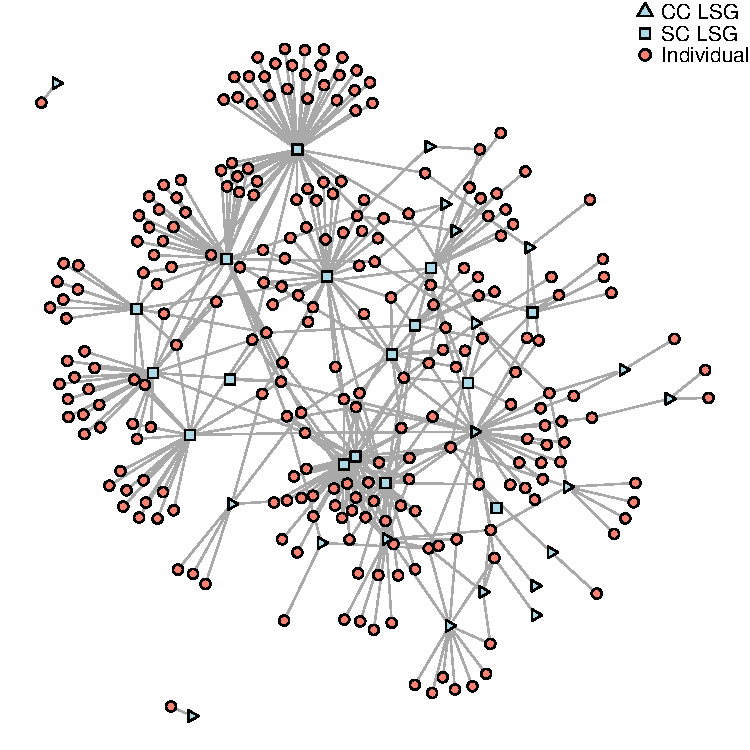
\includegraphics[width=3.5in]{LSG_full}
\par\end{centering}
\caption{The Central Committee (CC) and the State Council (SC) LSGs.}
\label{fig:lsgNet}
\end{figure}
\par\end{center}

Since more powerful CCP elites are more likely to be affiliated with more LSGs, we start by using a count model of LSG membership, in particular a negative-binomial regression. We compare three main models in accordance with our three ``who'' question. Our baseline model looks simply at individual elites' total level of appearances. This provides an approximate measure of popularity at the individual level (i.e., ``who are in charge''). The second model includes both total appearances and coappearances with Xi, attempting to capture impacts of the dyadic joint activities with Xi on LSG appointments (i.e., ``who do I work with''). We then turn to the latent angle distance an elite has with Xi, which takes into account the indirect ways an elite is connected to Xi (i.e., ``who are my friends'').

\begin{table}[!ht]
\centering
\caption{Negative binomial regressions on appointment to LSGs.}
\label{tab:xiMods}
\begin{tabular}{ l D{.}{.}{2}D{.}{.}{2}D{.}{.}{2} }
\hline\hline
  & \multicolumn{ 1 }{ c }{ Total Appearances } & \multicolumn{ 1 }{ c }{ Total Appearances } & \multicolumn{ 1 }{ c }{ Total Appearances } \\
  & \multicolumn{ 1 }{ c }{  } & \multicolumn{ 1 }{ c }{ \& Coappearances } & \multicolumn{ 1 }{ c }{ \& Latent Distance } \\ \hline
(Intercept)               & -0.02                     & -0.07                     & -0.23                    \\
                          & (0.16)                    & (0.17)                    & (0.18)                   \\
Total Appearances         & 0.01 ^{***}                & 0.02 ^{*}            & 0.01 ^{**}                  \\
                          & (0.00)                    & (0.01)                    & (0.00)                   \\
% Theta                     & 0.61 ^{***}               & 0.64 ^{***}               & 0.69 ^{***}              \\
%                           & (0.18)                    & (0.19)                    & (0.20)                   \\
Coappearances with Xi     &                           & -0.08                     &                          \\
                          &                           & (0.07)                    &                          \\
Latent Distance from Xi   &                           &                           & -0.80 ^{***}              \\
                          &                           &                           & (0.28)                    \\
%  $N$                       & 111                       & 111                       & 111                      \\
% AIC                       & 335.98                    & 336.57                    & 331.58                   \\
% BIC                       & 368.49                    & 379.92                    & 374.93                   \\
% $\log L$                 & -155.99                   & -152.28                   & -149.79                   \\
\hline\hline
 % \multicolumn{4}{l}{\footnotesize{Standard errors in parentheses}}\\
\textit{Note:} & \multicolumn{3}{r}{\footnotesize{$^*$ significant at $p<.10$; $^{**} p<.05$; $^{***} p<.01$}}
\end{tabular}
 \end{table}

The results of our first three models are reported in Table~\ref{tab:xiMods}. First, our baseline model suggests that elites' total appearances matter in LSG appointments. Those ``who are in change'' do attend more LSGs. Second, as shown in the coappearance model, simply joining Xi in same political events (i.e., those ``who work with Xi'') does not significantly matter in terms of LSG appointments. In fact, this relationship weakly points in the \emph{opposite} direction. This supports our earlier contention that simply focusing on ``who do I work with'' could mask latent relations between elites. Finally, in contrast to coappearances, the latent distance measure is significant and in the predicted direction. Elites who are closer to Xi in the latent space (i.e., those ``who are Xi's friends'') are seated on more LSGs.

In Figure~\ref{fig:effects}, we show the expected number of LSGs an elite with an average number of total appearances would be appointed to based on their latent distance from Xi, for that elite, moving from the closest angle distance observed to the furthest is associated with a drop in LSG appointment of about 1.5.

\noindent \begin{center}
\begin{figure}[H]
\noindent \begin{centering}
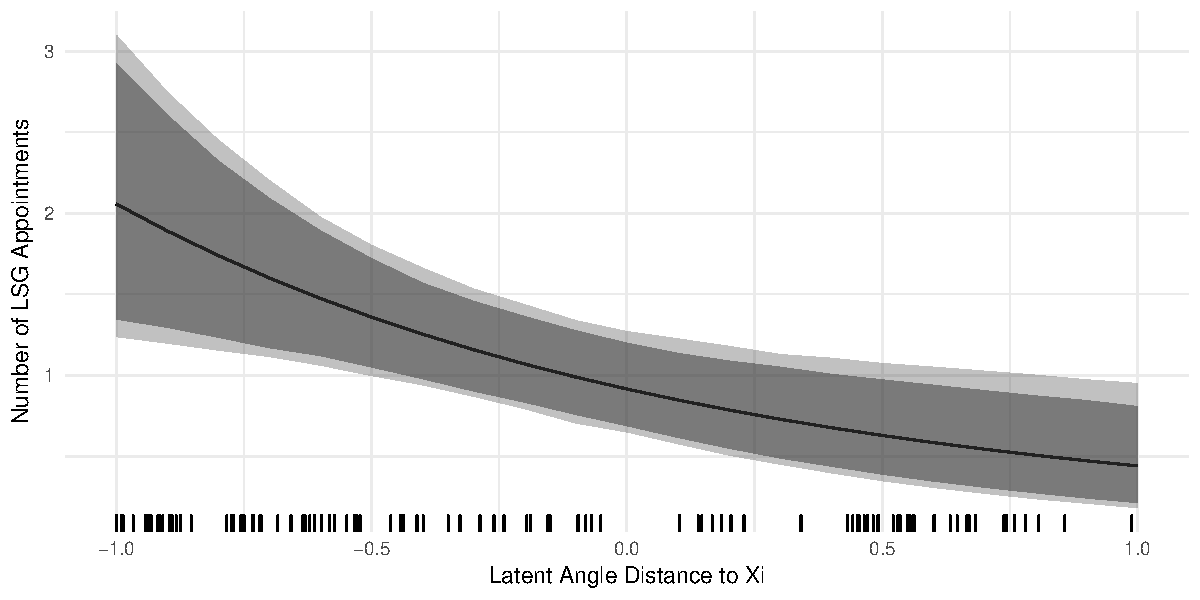
\includegraphics[width=1\textwidth]{effects}
\par\end{centering}
\caption{Estimated effect on number of LSG appointments based on latent distance to Xi.}
\label{fig:effects}
\end{figure}
\par\end{center}

While our measure of Chinese latent proximity conforms to our theoretical expectations in terms of conventional statistical significance, an important test is whether it improves our ability to predict appointments in an out-of-sample context. To do this, we divide Chinese elites into 20 groups at random, and in each case predict how many LSGs an elite in that group will be appointed to using a model fit on the other 19 groups. We do this for each of our three main models and report performance metrics in Table~\ref{tab:xiModsPerf}. To evaluate performance we use the root-mean-square error (RMSE) and proper scoring rules. Scoring rules evaluate forecasts through the assignment of a numerical score based on the predictive distribution and on the actual value of the dependent variable. \citet{czado:etal:2009} discuss a number of such rules that can be used for count data: Brier, Logarithmic, and Spherical scores. For each of these rules, lower values on the metric indicate better performance. We find the model using latent angle difference notably outperforms the models that only use total and coappearances across each of these metrics. This highlights that by accounting for indirect ties using the coappearance data we are able to better predict promotion to the Leading Small Groups than by looking at direct dyadic ties alone.

\begin{table}[ht]
\centering
\begin{small}
\caption{Out-of-sample performance on scoring rule metrics for models from Table~\ref{tab:xiMods}.}
\label{tab:xiModsPerf}
  \begin{tabular}{lcccc}
  \\[-1.8ex]\hline
  \hline \\[-1.8ex]
  Model & Logarithmic & Brier & Spherical & RMSE\\    \hline \\[-1.8ex]
Total Appearance & 1.77 & -0.36 & -0.64 & 1.89 \\
Total and Coappearance & 1.77 & -0.38 & -0.66 & 1.84 \\
Total Appearance and  & \multirow{2}{*}{1.73} & \multirow{2}{*}{-0.46} & \multirow{2}{*}{-0.86} & \multirow{2}{*}{1.74} \\
  \;\;\; Latent Distance to Xi &  &  &  &  \\
    \hline
 \hline \\[-1.8ex]
\end{tabular}
\end{small}
\end{table}

Finally, as emphasized by \citet{Huhe2018a}, there are marked structural differences between CC LSGs and SC LSGs. While CC LSGs are highly centralized, reflecting Xi's power grip the party, SC LSGs are far more decentralized and driven more by specific needs of policy collaboration. It is thus reasonable to expect while distances from Xi better predict CCP elites appointment in CC LSGs, distances from Li are more pronounced in SC ones. To probe these differences, we run a bivariate probit analysis, which estimates the likelihood that an elite will be appointed to any CC or SC LSGs jointly.

From Table~\ref{tab:bivarProbit}, we see that latent distance from Xi has a negative effect on the likelihood of appointment to CC LSGs, but being proximate to Xi in this latent social space has no clear effect on appointment to SC LSGs. Conversely, distance from Li is associated with a lowered likelihood of appointment to SC LSGs, but not the CC ones. These findings point to some interesting power-sharing patterns in the CCP regime. While Xi dominates the more important CC LSGs, Li preserves substantial influences over implementing key polices. The ability to distinguish between promotion to CC and SC LSGs renders more support for our approach to approximating the latent affinities between CCP elites.

\noindent \begin{center}
\begin{table}[H]
\caption{Bivariate probit analyses of CC and SC LSGs.}
\label{tab:bivarProbit}
\small
\centering
  \begin{tabular}{@{\extracolsep{0pt}} l D{.}{.}{2.2} D{.}{.}{2.2} D{.}{.}{2.2} D{.}{.}{2.2}  }
 \\[-1.8ex]\hline
 \hline \\[-1.8ex]
 \\[-1.8ex] & \multicolumn{2}{c}{Latent Distance to Xi} & \multicolumn{2}{c}{Latent Distance to Li}\\
 \\[-1.8ex] & \multicolumn{1}{c}{CC} & \multicolumn{1}{c}{SC} & \multicolumn{1}{c}{CC} & \multicolumn{1}{c}{SC} \\
 \hline
 & & & & \\
 Total appearances     & 0.05^{***} &-0.00     & 0.06^{***} &-0.00 \\
                       &(0.02)      &(0.00)     &(0.02)      &(0.00)\\
 Latent distance to Xi &-0.62^{**}  &-0.26       &            & \\
                       & (0.29)      &(0.23)      &            &\\
 Latent distance to Li &            &            &-0.34       &-1.86^{***}\\
                       &            &            &(0.36)      &(0.40)\\

 & & & & \\
 Intercept 1 & \multicolumn{2}{c}{$-1.20^{***}$} & \multicolumn{2}{c}{$-1.19^{***}$}\\
             & \multicolumn{2}{c}{(0.19)}        & \multicolumn{2}{c}{(0.21)}\\
 Intercept 2  & \multicolumn{2}{c}{$-0.70^{***}$} & \multicolumn{2}{c}{$-1.34^{***}$}\\
             & \multicolumn{2}{c}{(0.15)}        & \multicolumn{2}{c}{(0.23)}\\
 Intercept 3 & \multicolumn{2}{c}{$0.93^{**}$}   & \multicolumn{2}{c}{$0.91^{**}$}\\
             & \multicolumn{2}{c}{(0.02)}        & \multicolumn{2}{c}{(0.44)}\\
 & & & & \\
 \hline
 \hline \\[-1.8ex]
 \textit{Note:}  & \multicolumn{4}{r}{$^{*}p<$0.1; $^{**}p<$0.05; $^{***}p<$0.01} \\
 \end{tabular}
\end{table}
\par\end{center}

\section*{Conclusion and discussion}

In this study, we propose a latent factor framework to exploring elite networks. We treat elite power-sharing as a latent space, and we argue that we can approximate this space by studying elites' appearances in various political events (i.e., power foci). Specifically, we highlight three crucial questions in this approximation: who are in charge, who do I work with, and who are my friends. We further examine how this approach could improve our understanding of such pivotal informal institutions as LSGs. Our tests show that accounting for indirect ties between elites greatly improves our prediction of LSG appointments. Specifically, our latent distance measure notably outperforms measures that simply look at individual power (who are in charge) and dyadic relationships (who do I work with). As an additional demonstration of the measure's efficacy, we also find that it helps reveal CCP's more nuanced power-sharing arrangements. While the proximity to Xi helps to explain LSGs of the Central Committee, it is the latent distances from Li that better explain those of the State Council.

By introducing this framework, our study presents a possible avenue to synthesize different aspects of elite power-sharing in authoritarian regimes. It not only encompasses positional status of individual elites, but also incorporates how they are interrelated. This allows us to develop a systematic view about the inherent and uneasy tensions among authoritarian elites. As long noted by \citet{Pye1995}, ``Chinese politics operated in an atmosphere of tension in which everyone sensed the need always to be careful and calculating about what was done or said'' (p. 36). The three who questions proposed in this study then help highlight their key heuristics. Particularly, our emphasis on the question of ``who are our friends'' suggests that we need to move beyond just examining the direct ties actors share.

Last, studies of elite politics in authoritarian regimes have also been long plagued with data paucity. Our study points to an alternative data source, appearance data, that could complement existing data like media coverage and biographical archives. Such data not only is dynamic, it also sheds light on the actual realization of power relationship as emphasized by \citet{Dahl1961}. As a preliminary exploration, our study is inevitably limited, and more systematic are called for to improve collection and analysis of such data.  First, in approximating the latent affinities among CCP elites, we treat their appearances between 2013 and 2017 as cross-sectional, which could mask temporal shifts.  With more systematic data collection, future studies can benefit from longitudinal explorations of the evolution of the CCP elite network.  Second, we focus mainly on the latent relationship between the CCP elites.  This leaves a number of avenues for future research:  For example, is attendance at some events more important than others?  Is attendance at some events conducive to a future promotion?  Future studies can also benefit from adopting a bipartite framework, simultaneously looking at the characteristics and latent positions of both events and elites.  Finally, we could also develop a better understanding of elite politics by disentangling the relationship between elites' public appearances and nodal characteristics such as home province, educational institutions, and previous work experience.

\newpage{}

\begin{spacing}{1}

\bibliographystyle{apsr}
\bibliography{narisbio}

\end{spacing}

\par\end{flushleft}
\end{document}


% Provided with the two clusters as shown in Figure~\ref{fig:uv}, we further model LSG appointments based on distance to Li Keqiang. The results are presented in Table~\ref{tab:xiliMods}. We find that latent distance from Li is similarly associated with a lower probability of appointment to LSGs. However, combining the two distance measures results in a model that has ambiguous effects. One reason is that for most members of the party, distance from Xi and Li are highly collinear. Importantly however, they differ for some individuals. As shown in Table~\ref{tab:xiliModsPerf}, inclusion of latent distance to Li does not necessarily improve model performance out of sample. This implies that, for elites whose distances to Xi and Li diverge, adding information about proximity to Li actually hurts the model's performance.

% \begin{table}[!ht]
% \centering
% \caption{Negative binomial regressions on appointment to LSGs by relationship to Xi and Li}
% \label{tab:xiliMods}
% \begin{tabular}{ l D{.}{.}{2}D{.}{.}{2} }
% \hline \hline
%   & \multicolumn{ 1 }{ c }{ Xi Only } & \multicolumn{ 1 }{ c }{ Li Only } \\ \hline
%  %                       & Xi Only      & Li Only     \\
% (Intercept)             & -0.23        & -0.59 ^{***} \\
%                         & (0.18)       & (0.21)      \\
% Total Appearances       & 0.01 ^{**}      & 0.01 ^{***}  \\
%                         & (0.00)       & (0.00)      \\
% Latent Distance from Xi & -0.80 ^{***}  &             \\
%                         & (0.28)       &             \\
% % Theta                   & 0.69 ^{***}  & 0.93 ^{**}  \\
% %                         & (0.20)       & (0.32)      \\
% Latent Distance from Li &              & -1.42 ^{***}\\
%                         &              & (0.37)       \\
% %  $N$                     & 111          & 111         \\
% % AIC                     & 331.58       & 323.30      \\
% % BIC                     & 374.93       & 366.66      \\
% % $\log L$               & -149.79      & -145.65      \\
% \hline\hline
%  % \multicolumn{3}{l}{\footnotesize{Standard errors in parentheses}}\\
%  \multicolumn{3}{r}{\textit{Note: } \footnotesize{$^*$ significant at $p<.10$; $^{**} p<.05$; $^{***} p<.01$}}
% \end{tabular}
%  \end{table}

% \noindent \begin{center}
% \begin{table}[H]
% \caption{Out-of-sample performance on scoring rule metrics for models shown in Table~\ref{tab:xiliMods}}
% \label{tab:xiliModsPerf}
% \small
% \centering
%   \begin{tabular}{lccccc}
%   \\[-1.8ex]\hline
%   \hline \\[-1.8ex]
%    & & & & Dawid & \\
%    Model & Logarith & Brier & Spherical & Sebastiani & RMSE\\    \hline \\[-1.8ex]
% Total Appearance and Latent Distance to Xi & 1.73 & -0.46 & -0.86 & 2.66 & 1.74 \\
% Total Appearance and Latent Distance to Li & 1.64 & -0.51 & -0.96 & 2.41 & 1.90 \\
%  \hline \\[-1.8ex]
% \end{tabular}
% \noindent \begin{raggedright}
% \emph{Note}: For each of the metrics, lower values indicate better
% performance. For more details about scoring rules, see the Appendix.
% \par\end{raggedright}
% \end{table}
% \par\end{center}

% \noindent \begin{center}
% \begin{table}[H]
% \caption{Bivariate probit analyses of CC and SC LSGs}
% \label{tab:bivarProbit}
% \small
% \centering
%   \begin{tabular}{@{\extracolsep{0pt}} l D{.}{.}{2.2} D{.}{.}{2.2} D{.}{.}{2.2} D{.}{.}{2.2} D{.}{.}{2.2} D{.}{.}{2.2} D{.}{.}{2.2} D{.}{.}{2.2} D{.}{.}{2.2} D{.}{.}{2.2}}
%  \\[-1.8ex]\hline
%  \hline \\[-1.8ex]
%  \\[-1.8ex] & \multicolumn{2}{c}{Model 6} & \multicolumn{2}{c}{Model 7} & \multicolumn{2}{c}{Model 8} & \multicolumn{2}{c}{Model 9} & \multicolumn{2}{c}{Model 10}\\
%  \\[-1.8ex] & \multicolumn{1}{c}{CC} & \multicolumn{1}{c}{SC} & \multicolumn{1}{c}{CC} & \multicolumn{1}{c}{SC} & \multicolumn{1}{c}{CC} & \multicolumn{1}{c}{SC} & \multicolumn{1}{c}{CC} & \multicolumn{1}{c}{SC} & \multicolumn{1}{c}{CC} & \multicolumn{1}{c}{SC} \\
%  \hline
%   & & & & & & & & & & \\
%  Total appearances     & 0.06^{***} & 0.00      &            &            &            &            & 0.05^{***} &-0.00     & 0.06^{***} &-0.00 \\
%                        &(0.02)      &(0.00)     &            &            &            &            &(0.02)      &(0.00)     &(0.02)      &(0.00)\\
%  Latent distance to Xi &            &            &-1.19^{***} &-0.27       &            &            &-0.62^{**}  &-0.26       &            & \\
%                        &            &            &(0.27)      &(0.22)      &            &            &(0.29)      &(0.23)      &            &\\
%  Latent distance to Li &            &            &            &            &-0.78^{**}  &-1.81^{***} &            &            &-0.34       &-1.86^{***}\\
%                        &            &            &            &            &(0.32)      &(0.39)      &            &            &(0.36)      &(0.40)\\

%  & & & & & & & & & & \\
%  Intercept 1 & \multicolumn{2}{c}{$-1.08^{***}$} & \multicolumn{2}{c}{$-0.94^{***}$} & \multicolumn{2}{c}{$-0.77^{***}$} & \multicolumn{2}{c}{$-1.20^{***}$} & \multicolumn{2}{c}{$-1.19^{***}$}\\
%              & \multicolumn{2}{c}{(0.18)}        & \multicolumn{2}{c}{(0.18)}        & \multicolumn{2}{c}{(0.17)}        & \multicolumn{2}{c}{(0.19)}        & \multicolumn{2}{c}{(0.21)}\\
%  Intercept 2 & \multicolumn{2}{c}{$-0.65^{***}$} & \multicolumn{2}{c}{$-0.69^{***}$} & \multicolumn{2}{c}{$-1.36^{***}$} & \multicolumn{2}{c}{$-0.70^{***}$} & \multicolumn{2}{c}{$-1.34^{***}$}\\
%              & \multicolumn{2}{c}{(0.14)}        & \multicolumn{2}{c}{(0.14)}        & \multicolumn{2}{c}{(0.23)}        & \multicolumn{2}{c}{(0.15)}        & \multicolumn{2}{c}{(0.23)}\\
%  Intercept 3 & \multicolumn{2}{c}{$0.91^{**}$}   & \multicolumn{2}{c}{$0.90^{**}$}   & \multicolumn{2}{c}{$0.51$}        & \multicolumn{2}{c}{$0.93^{**}$}   & \multicolumn{2}{c}{$0.91^{**}$}\\
%              & \multicolumn{2}{c}{(0.40)}        & \multicolumn{2}{c}{(0.38)}        & \multicolumn{2}{c}{(0.37)}        & \multicolumn{2}{c}{(0.02)}        & \multicolumn{2}{c}{(0.44)}\\
%   & & & & & & & & & &\\
%  \hline
%  \hline \\[-1.8ex]
%  \textit{Note:}  & \multicolumn{10}{r}{$^{*}p<$0.1; $^{**}p<$0.05; $^{***}p<$0.01} \\
%  \end{tabular}
% \end{table}
% \par\end{center}
